\documentclass[a4paper]{article}
\usepackage{geometry}
\geometry{a4paper, portrait, margin=1in}
\usepackage[english]{babel}
\usepackage[utf8]{inputenc}
\usepackage{natbib}
\usepackage{graphicx}
\usepackage{fancyhdr}
\usepackage{array}
\usepackage{tabu}
\usepackage{listings}
\usepackage[export]{adjustbox}

\title{Computing GCSE Coursework}
\author{\\ \\ \\ \\ Thomas Bass\\Candidate 4869\\Centre 52423\\OCR A453 Programming Project\\\\ Word Count 1678 \\\\\ Made with \LaTeX}
\date{2016-2017}


\pagestyle{fancy}
\fancyhf{}
\rhead{Computing GCSE Coursework}
\chead{Candidate 4869}
\lhead{Thomas Bass}
\rfoot{Page \thepage}

\begin{document}

\maketitle
\pagebreak
\renewcommand*\contentsname{Summary}
\tableofcontents
\pagebreak
%%%%%%%%%%%%%%%%%%%%%%%%%%%%%%%%%%%%%%%%%%%%%%%%%%%%%%%%%%%%%%%%%%%%%%%%%%%%
\section{Objectives}

\subsection{Task 1}
\begin{enumerate}
\item{Take an input and verify that it is 8 or 7 numerical digits}
\item{Calculate the 8th check digit:}
\item[~a]{Multiply the first 7 numbers alternately by 3,1}
\item[~b]{Total these results}
\item[~c]{Subtract this sum from its nearest highest multiple of 10}
\item{Compare this to the given 8th number, or complete the 7-digit number}
\end{enumerate}

\subsection{Task 2}
\begin{enumerate}
\item{Take an input and validate that it is 8 numerical digits}
\item{Connect to a SQL database and run a query}
\item{Collect and display the results}
\item{Update the database with the customer?s order}
\item{Print a receipt}
\item{Cope with SQL errors}
\end{enumerate}

\subsection{Task 3}
\begin{enumerate}
\item{Scan a database and find stock to order}
\item{Create a receipt of the order}
\item{Update the database with the updated stock level}
\item{Cope with any SQL errors}
\end{enumerate}

\pagebreak

%%%%%%%%%%%%%%%%%%%%%%%%%%%%%%%%%%%%%%%%%%%%%%%%%%%%%%%%%%%%%%%%%%%%%%%%%%%%
\section{Test Plan}

\subsection{Task 1}
\begin{enumerate}
\item{Input strings of incorrect length. If rejected, it passes.}
\item[~]{Test data: \verb|12345|}
\item[~]{Test data: \verb|1234567890|}
\item{Input strings of letters. If rejected, it passes.}
\item[~]{Test data: \verb|abcdefg|}
\item{Get program to run a valid input. Print out totals at each stage, and check them manually. If they are the same, it passes.}
\item[~]{Test data: \verb|13245627|}
\item[~i.]{Manually add the totals of a valid input. If they are the same, it passes.}
\item[~ii.]{Manually round the total to the highest 10. If it is the same, it passes.}
\item[~iii.]{Manually collect the distance rounded. If it is the same, it passes.}
\item{Run the program with a GTIN number taken from a product. If it correctly calculated and verified, it passes.}
\end{enumerate}

\subsection{Task 2}
\begin{enumerate}
\item{Input strings of incorrect length. If rejected, it passes.}
\item[~]{Test data: \verb|12345|.}
\item[~]{Test data: \verb|1234567890|.}
\item{Input strings of letters. If rejected, it passes.}
\item[~]{Test data: \verb|abcdefg|.}
\item{Input a valid string to search. If product found, it passes.}
\item[~]{Test data: \verb|11440529|.}
\item{Manually check that the program has displayed the correct stock level and information. If it does, it passes.}
\item[~]{Stock info: 50 in stock for \#\verb|11440529| (red paint 100ml).}
\item{Order a quantity of the product. If the program updates the stock levels, it passes.}
\item[~]{Test data: order 5 x QTY of \#\verb|11440529| (red paint 100ml).}
\item{Complete a full order. If the program displays a receipt with the correct values, it passes.}
\item[~]{Test data: order 5 x QTY of \#\verb|11440529| (red paint 100ml) AND}
\item[~]{6 x QTY of \#\verb|11509493| (blue paint 100ml).}
\item[~]{Expected result: 5 x \#\verb|11509493| = \pounds9.95 AND 6x \#\verb|11509493| = \pounds11.94, total:  \pounds21.90 .}
\item{Provide the program with invalid values (such as ordering negative values). If the program rejects these, it passes.}
\item[~]{Test data: -3 x QTY \#\verb|11509493|.}
\item[~]{Expected result: error and re-input.}
\item[~]{Test data 0 x QTY \#\verb|11509493|.}
\item[~]{Expected result: error and re-input.}
\item[~]{Test data: 100 x QTY \#\verb|11509493|.}
\item[~]{Expected result: not enough stock, re-input.}
\end{enumerate}

\subsection{Task 3}
\begin{enumerate}
\item{Edit database for reduced stock. If reduced stock is identified, it passes.}
\item[~]{Test data: Edit a stock level to -10 of stock level.}
\item[~]{Print receipt.}
\item{Edit database for reduced stock. If a human-readable receipt is produced, it passes.}
\item[~]{Test data: Edit two stock levels to -10 of stock level.}
\item[~]{Print receipt.}
\item{Complete order for reduced stock. If the database updated, it passes.}
\item[~]{Continue from test area 2, and update database.}
\item[~]{Check database manually.}
\item{If the program handles SQL errors, it passes.}
\item[~]{Attempt to update from more than stock level.}
\end{enumerate}


\pagebreak

%%%%%%%%%%%%%%%%%%%%%%%%%%%%%%%%%%%%%%%%%%%%%%%%%%%%%%%%%%%%%%%%%%%%%%%%%%%%
\section{Pseudocode}
\subsection{Task 1}
\begin{lstlisting}
START
User INPUT choice for calculate or verify	
IF Calculate:
Number Length is 7
  INPUT GTIN
  CALL Verify function
ELSE IF Verify:
  Number Length is 8
  INPUT GTIN
  CALL verify Function
ENDIF
ENDIF
Verify Function:
  IF GTIN length = Length AND is all numeric:
    For a loop of 7 by step of 2:
      total = total+(GTIN [counter]*3)
      IF counter =6:
        Round total UP to nearest multiple of 10
        result = roundedNumber - total
          If Length = 7:
            Print result
            ASK User to repeat
          ELSE
            If GTIN at position Length = result:
              Print GTIN is a valid number
              ASK User to repeat
            ELSE:
              Print GTIN is an invalid number
              ASK User to repeat
            ENDIF
      ELSE
        Multiply GTIN at position of counter+1 by 1 and add to total
      ENDIF
  ELSE
    Print error and return to GTIN input
  ENDIF
END
\end{lstlisting}
\pagebreak

\subsection{Task 2}
\begin{lstlisting}
START
User INPUT GTIN number
IF GTIN is numerical AND GTIN = 8 charachters:
  Search Database for GTIN number
  IF result found:
    User INPUT quantity to order
    IF quantity > 0 AND quantity <= stock available
      PRINT receipt with total cost (cost per item * quantity ordered)
      Update Database with new stock (stock available a quantity ordered)
      User INPUT choice to order more items
      IF choice = yes:
        Add to order list and return to GTIN INPUT
      ELSE
        PRINT final receipt (order list) and end program
      ENDIF
    ELSE
      Return to Quantity INPUT
    ENDIF
  ELSE
    Return to GTIN INPUT
  ENDIF
ELSE
  Return to GTIN INPUT	
ENDIF
END
\end{lstlisting}
\

\subsection{Task 3}
\begin{lstlisting}
START
Connect to SQL Database
Search database:
  IF stock level < target stock level:
  RETURN results
PRINT results
APPEND results to order list
IF order complete:
  UPDATE database:
  stock level = target stock level
ELSE
  END
ENDIF
END
\end{lstlisting}

\pagebreak

%%%%%%%%%%%%%%%%%%%%%%%%%%%%%%%%%%%%%%%%%%%%%%%%%%%%%%%%%%%%%%%%%%%%%%%%%%%%

\section{Data Structure}
\subsection{Task 1}
\begin{center}
\begin{tabular}{ | m{13em} | m{16em} | }
  \hline
  Variable Name & Variable Description	\\ [0.5ex] 
  \hline\hline
  \verb|ask| & The choice wether the user wants to verify or calculate \\
  \hline
  \verb|gtin| & The GTIN number used \\
  \hline
  \verb|length| & The length the GTIN should be \\
  \hline
  \verb|total| & The running total of all the multiplications \\
  \hline
  \verb|checkdig| & The 8th digit in a verification \\
  \hline
  \verb|rounded| & \verb|total| Rounded up to the nearest 10 \\ 
  \hline
  \verb|result| & The 8th digit as the program calculates it \\
  \hline
  \verb|again| & The choice of wether the user wants to run the program again \\
  \hline 
\end{tabular}
\end{center}

\subsection{Task 2}
\begin{center}
\begin{tabular}{ | m{13em} | m{16em}| m{14em} | } 
 \hline
 Variable Name & Variable Description & Value \\ [0.5ex] 
 \hline\hline
 \verb|con| and \verb|cur| & Connections to SQL database & N/A \\ 
 \hline
 \verb|var| & User Input GTIN number & User Defined \\
 \hline
 \verb|results| & Fetchall results from SQL query & N/A (list) \\
 \hline
 \verb|product| & Equal to \verb|results|, reformatted & Equal to \verb|results| \\
 \hline
 \verb|sizeName| and \verb|sizeNameRaw| & Variables used to format the name of the product & Name of product selected \\
 \hline
 \verb|QtyToOrder| & User Input quantity ordered & User Defined \\
 \hline
 \verb|NewStockAvab| & Variable used to update the SQL database with the new stock levels & Stock Available minus \verb|QtyToOrder| \\ 
 \hline
 \verb|costOfOrder| & Total cost of order & Price of product*\verb|QtyToOrder| \\
 \hline
 \verb|currentOrderAddRaw| and \verb|currentOrderAdd| and \verb|currentOrder| & Variables used to format and append the order to the entire list of order (to print receipt) & N/A \\ [1ex] 
 \hline
\end{tabular}
\end{center}

\subsection{Task 3}
\begin{center}
\begin{tabular}{ | m{13em} | m{16em}| m{14em} | } 
  \hline
  Variable Name & Variable Description & Value \\ [0.5ex] 
  \hline\hline
  \verb|con| and \verb|cur| & Connections to SQL database & N/A \\
  \hline
  \verb|sql1| & SQL command for finding reduced stock levels & \verb|SELECT* FROM Inventory| \verb|WHERE StockAvab !=| \verb|Target Stock| \\
  \hline
  \verb|results| & Fetchall results from SQL query & N/A, List	\\
  \hline
  \verb|toOrder| & Value of how much stock needs to be ordered for each product & \verb|targetStock| - \verb|stockAvab| \\
  \hline
  \verb|sizeName| and \verb|sizeNameRaw| & Used to correctly format the product name & N/A \\
  \hline
  \verb|stockOrderAddRaw| and \verb|stockOrderAdd| and \verb|stockOrder| & Used to format the list of the stock update order & N/A \\
  \hline
  \verb|orderList| & Final order list & N/A \\
  \hline
  \end{tabular}
\end{center}

%%%%%%%%%%%%%%%%%%%%%%%%%%%%%%%%%%%%%%%%%%%%%%%%%%%%%%%%%%%%%%%%%%%%%%%%%%%%

\section{Development}
\subsection{Task 1}
For all my development, the code was written in Python's IDLE, an integrated development environment which comes packaged with Python installs.
\paragraph{Objective 1: Take an input and verify that it is 8 or 7 numerical digits}
\subparagraph{\texttt{start()} Function} ~ \par ~ \par
\noindent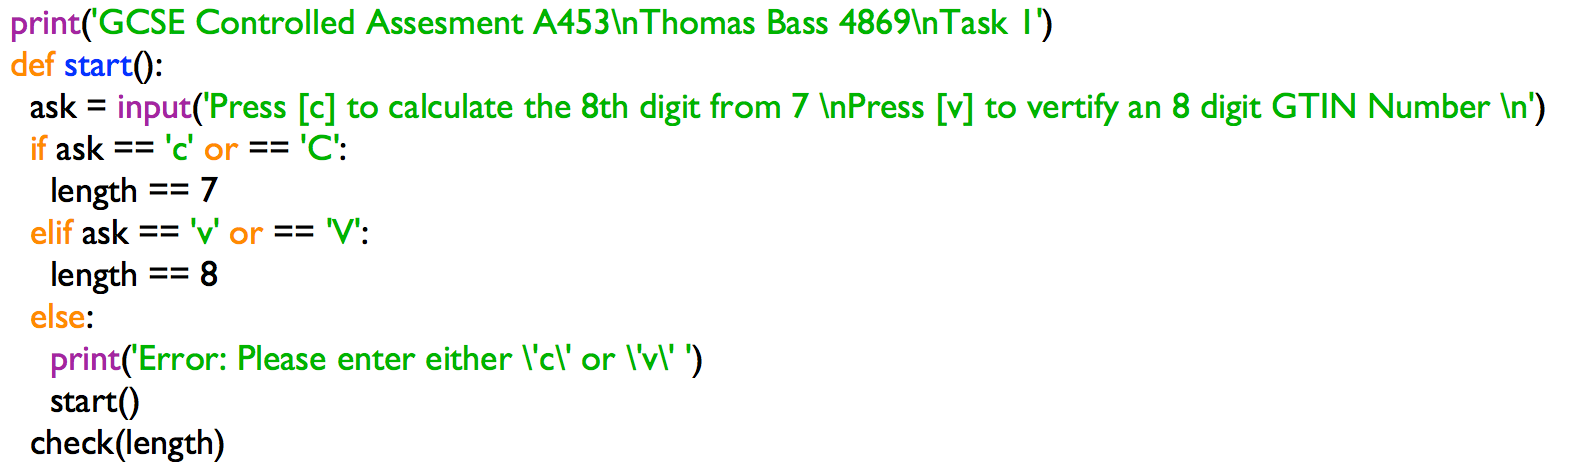
\includegraphics[width=1\textwidth, left, width=\linewidth, frame]{task1_start()functionDev.png}
This function takes a user input of 'ask' to decide if the user wants to either calculate the 8th GTIN digit from 7 digits (choice \verb|c|), or verify the 8th GTIN digit from 8 digits (choice \verb|v|). 
If the choice is \verb|c|, the program creates the variables \verb|gtin| and \verb|length|, and sets \verb|length| to 7. It then calls the \verb|check()| function carrying \verb|length| with it. \par
If the choice is \verb|v|, the program creates the variables \verb|gtin| and \verb|length|, and sets \verb|length| to 8. It then calls the \verb|check()| function carrying \verb|length| with it. \par
The first revision produced syntax errors on line 4 and 6. This is because the variable has to be re-stated after an \verb|or| condition. After this was corrected, the IDLE gave the following error: \par
\noindent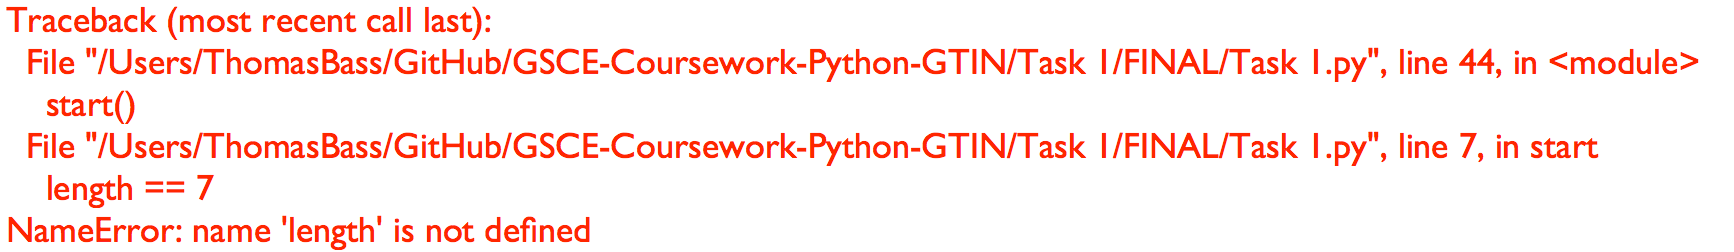
\includegraphics[width=1\textwidth, left, width=\linewidth, frame]{task1_start()functionDev2.png}
This error was produced as the incorrect operators were used in lines 5 and 7. The IDLE interpreted the code to compare \verb|length| to the number 7 (line 5) or 8 (line 7). These were then corrected to \verb|length = 7| and \verb|length = 8| respectively. The program then gave the following output: \par
\noindent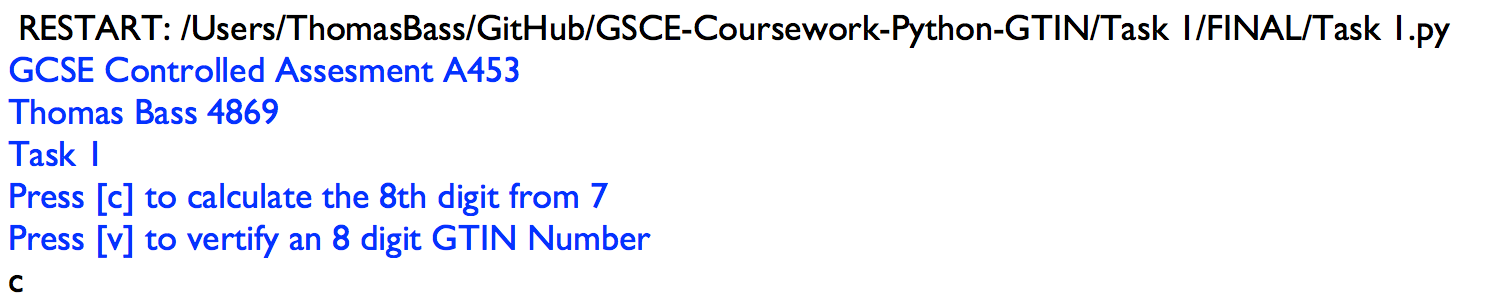
\includegraphics[width=0.9\textwidth, left, width=\linewidth, frame]{task1_start()functionDev3.png} \par
From the following code: \par
\noindent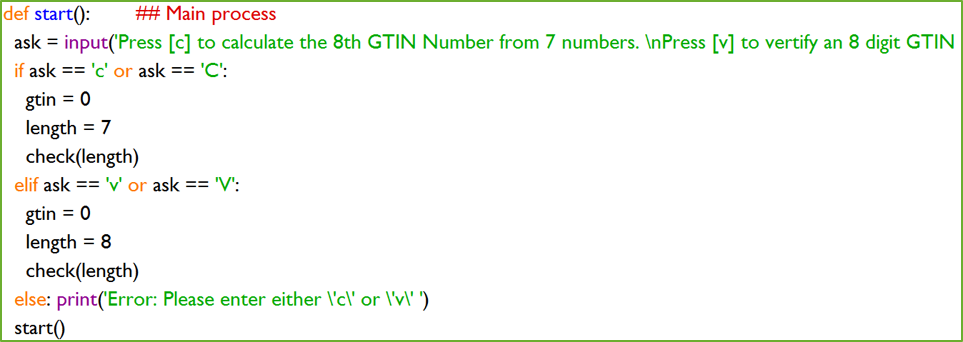
\includegraphics[width=0.7\textwidth, left]{task1_start()function.png} \par
This shows that the \verb|start()| function is working correctly
\newpage
\subparagraph{\texttt{check()} Function} ~ \par ~ \par
\noindent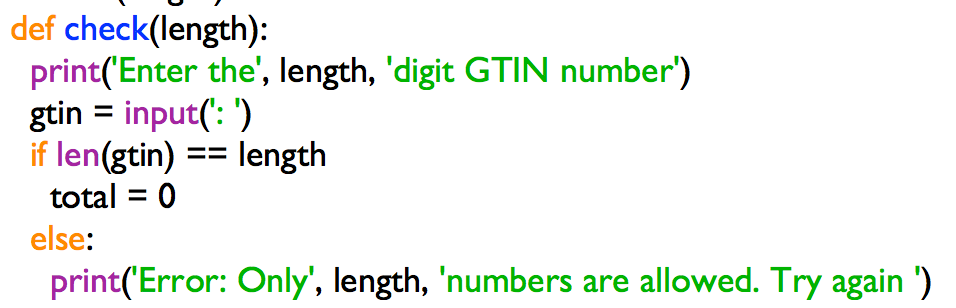
\includegraphics[width=0.5\textwidth, left, width=\linewidth, frame]{task1_check()functionDEV.png} \par
This function prints a statement asking the user for the \verb|length| length GTIN. It then takes the user input of \verb|gtin|. \par
If the length of \verb|gtin| is equal to \verb|length| and \verb|gtin.isnumeric| function is True (the variable is numerical) then it creates the variable \verb|total|. Else, it prints an error message, and returns to the \verb|check()| function. \par
The first revision gave a syntax error on line 4, as there was a missing colon. This was added, and the second revision ran, and rejected incorrect lengths, but allowed correct lengths including letters. The \verb|math| Python library provides the \verb|isnumeric| function that gives boolean \verb|False| if the variable carried contains characters other than numerical. This was used as \verb|if gtin.isnumeric() == True|. The program then gave the following output: \par
\noindent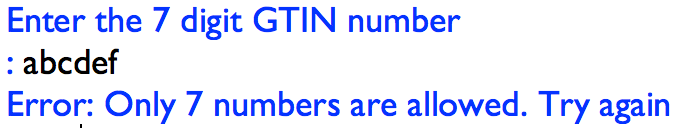
\includegraphics[width=0.5\textwidth, left, width=\linewidth, frame]{task1_check()functionDEV1.png} \par
The program worked and rejected invalid strings, but if the user had entered an invalid input, the program would reject it, but terminate the program. The code was then added after line 7 to call \verb|check(length)| after an invalid input. \verb|length| is carried so that the program does not have to re-start. The program then ran the following output: \par
\noindent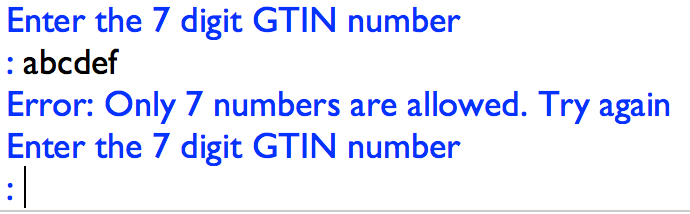
\includegraphics[width=0.5\textwidth, left, width=\linewidth, frame]{task1_check()functionDEV2.png} \par
With the following code: \par
\noindent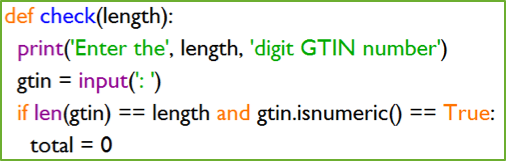
\includegraphics{task1_check()function2.png} ~ \par
\noindent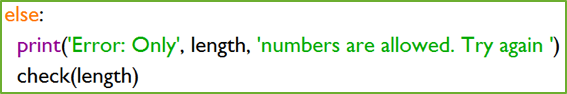
\includegraphics{task1_check()function3.png} ~\par
This shows that the program is correctly calling \verb|check(length)|, and is working correctly.
\newpage
\paragraph{Objective 2: Calculate the 8th check digit}
\subparagraph{Multiply the first 7 numbers alternately by 3,1} ~ \par ~ \par
\noindent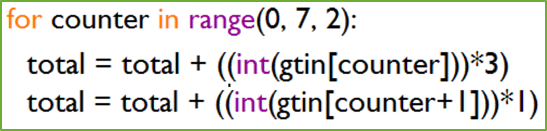
\includegraphics{task1_multiply1.png} ~\par
This snippet starts a loop for the value of \verb|counter|, which goes from 0 to 7, stepping by 2 each time. The counter could have gone 0 to 3 stepping by 1, but this would make it more complicated. The program then adds the following to \verb|total| : integer of: \verb|gtin| at position of \verb|counter| multiplied by 3. \par
\noindent It then adds to following to \verb|total| : integer of \verb|gtin| at position of \verb|counter+1| multiplied by 1.
\subparagraph{Total these results} ~\par
\noindent The program simply adds all of these calculations to \verb|total|
\subparagraph{Subtract this sum from its nearest highest multiple of 10} ~\par ~\par
\noindent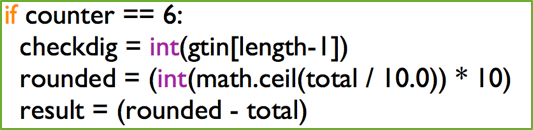
\includegraphics{task1_subtract1.png} ~\par
This snippet checks to see if the loop is on its final iteration (\verb|counter| = 6). It then sets \verb|checkdig| to the penultimate digit of \verb?gtin?. It then creates the variable \verb?rounded? and sets it to to the nearest highest multiple of 10 of \verb?total?. It then creates the variable \verb?result? and sets it to the result of \verb?rounded? - \verb?total?.
\paragraph{Objective 3: Compare this to the given 8th number, or complete the 7-digit number} ~\par ~\par
\noindent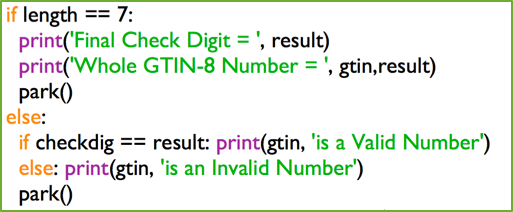
\includegraphics{task1_compare1.png} ~\par
In this section of code, if \verb?length? equals 7, the program prints the final check digit (\verb?result?), and also prints the whole calculated GTIN (\verb?gtin? and \verb?result?). It then calls the \verb|park()| function
Else, if \verb?checkdig? is equal to \verb?result?, it prints that \verb?gtin? is a valid number. Else, it prints that \verb?gtin? is an invalid number.
\subparagraph{\texttt{park()} Function} ~ \par ~ \par
The \verb|park()| function is used after a verification or calculation has been made, and allows the user to carry out more verifications or calculations without restarting the program. \par
\noindent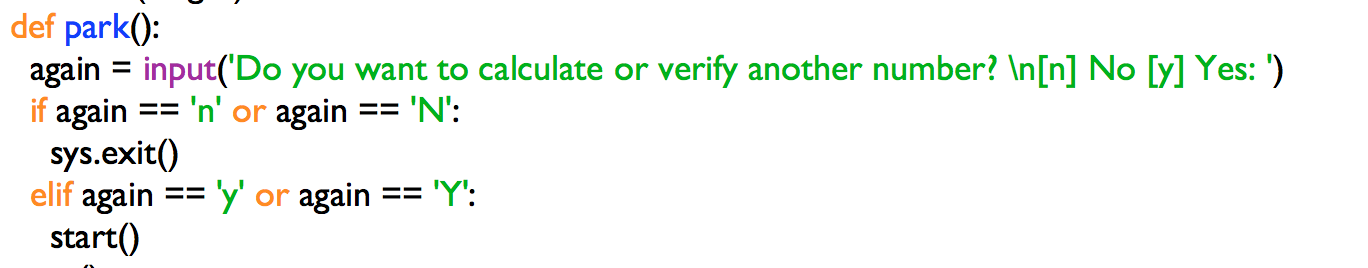
\includegraphics[width=0.7\textwidth, left, width=\linewidth, frame]{task1_park().png} \par
This program asks the user if they want to restart the program. If yet, it calls \verb|start()| function, and if no it ends the program. The \verb|sys| Python library provides the \verb|.exit()| function to terminate the program. In IDLE it simply ends it, but when compiled into command line it will close the window.


\newpage
\subsection{Task 2}
\paragraph{Objective 1: Take an input and validate that it is 8 numerical digits} ~\par ~\par
\noindent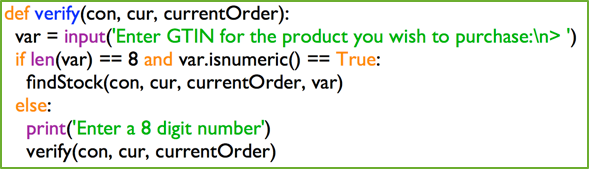
\includegraphics{task2_obj1_1.png} ~\par
This function takes the user input \verb?var?. If it is 8 digits long and \verb|var.isnumeric| function is True (the variable is numerical) , it calls findStock function, carrying \verb?con? and \verb?cur? (variables for SQL database connection), \verb?currentOrder?, and \verb?var?. Else, it prints an error message and returns to \verb|verify()| function.
\paragraph{Objective 2: Connect to a SQL database and run a query} ~\par ~\par
\noindent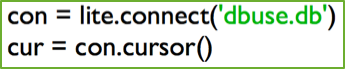
\includegraphics{task2_obj2_1.png} ~\par
This snippet uses the sqlite3 library to connect to the database file \verb?dbuse.db?. ~\par ~\par
\noindent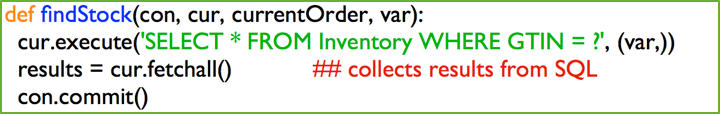
\includegraphics{task2_obj2_2.png} ~\par
The \verb|findStock()| function executes the SQL query to find the record in \verb?Inventory? where GTIN is equal to \verb?var?. It then sets the variable \verb?results? to the results of this query. ~\par
\paragraph{Objective 3: Collect and display the results} ~\par ~\par
\noindent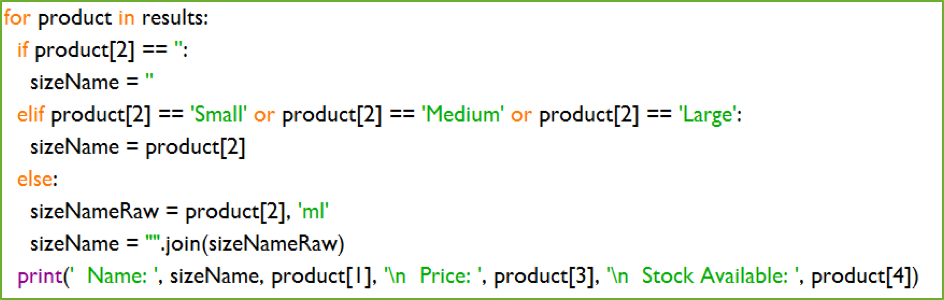
\includegraphics{task2_obj3_1.png} \par
This section of code formats the product name: If the product has no size, it displays the name. If it has a small/medium/large quantity, it appends that to the end. If it has a ml volume, it appends that to the front. It then prints the name of the product as product name, volume, price, stock available.
\newpage
\paragraph{Objective 4: Update the database with the customer's order} ~\par ~\par
\noindent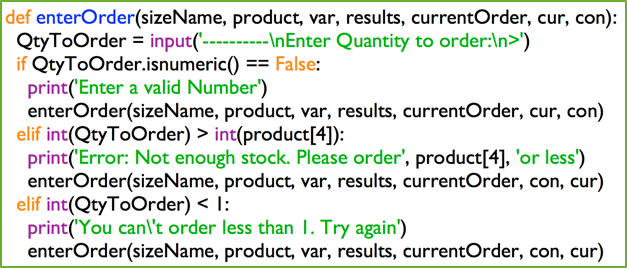
\includegraphics{task2_obj4_1.png} \par 
This section of \verb|enterOrder()| function ensures that the customer can only order more than 1, and less than or equal the number of stock available. ~\par ~\par
\noindent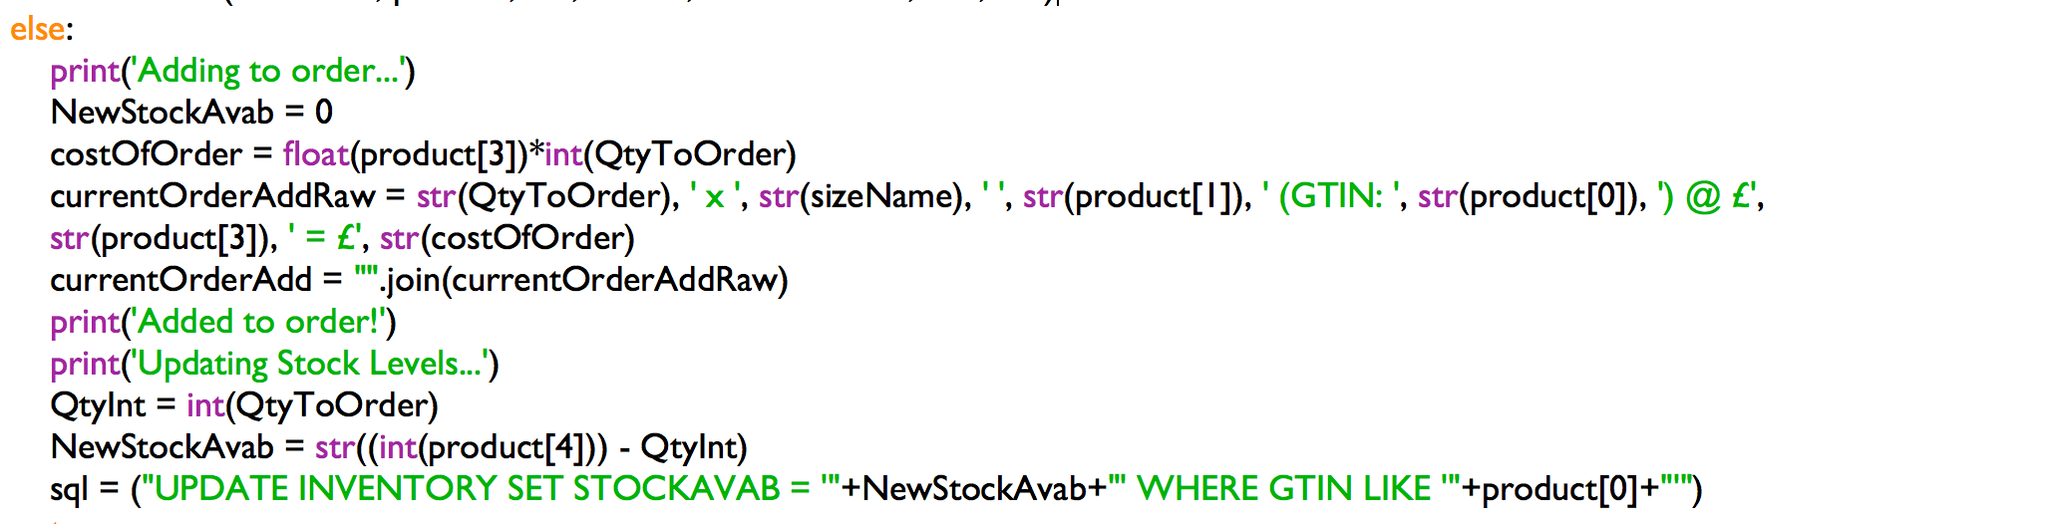
\includegraphics[width=0.8\textwidth, left, width=\linewidth, frame]{objective4_dev.png} \par
This section creates a verbose receipt, and makes an SQL query to update the database with the new stock levels. \par
When this was tested, it produced this output: \par
\noindent
\includegraphics[width=0.8\textwidth, left, width=\linewidth, frame]{obj4error.png} \par 
The calculation for the final cost was broken as Python can not read over a line break. The line break in line 5 and 6 was stopping the full calculation. This was fixed: \par
\noindent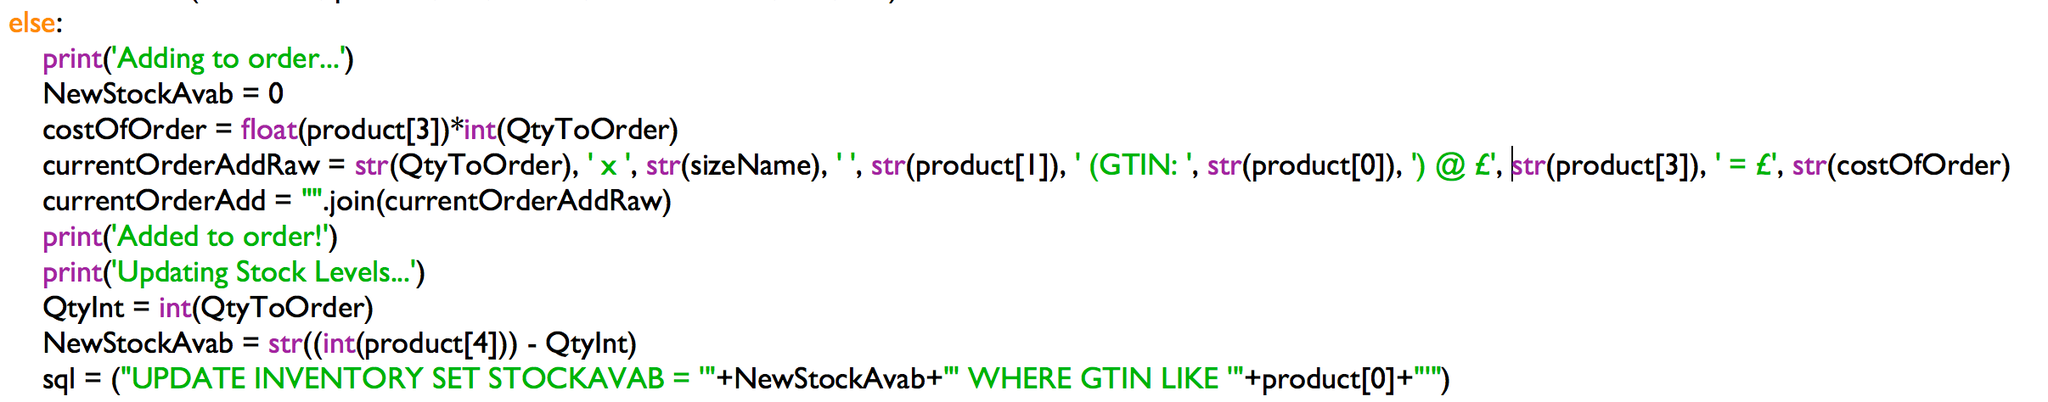
\includegraphics[width=0.8\textwidth, left, width=\linewidth, frame]{obj4fixed.png} \par 
The program was then tested to give the following correct output: \par
\noindent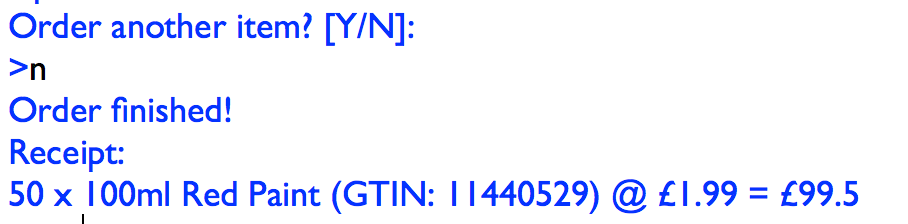
\includegraphics[width=0.8\textwidth, left, width=\linewidth, frame]{obj4fixedproof.png} \par 
\newpage
\paragraph{Objective 5: Print a receipt} ~\par ~\par
\noindent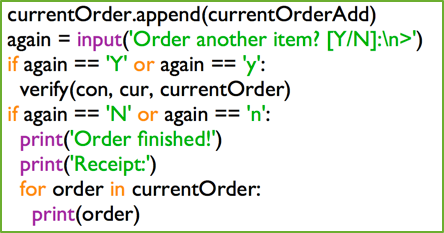
\includegraphics{task2_obj5_1.png} \par 
\paragraph{Objective 6: Cope with SQL errors} ~\par ~\par
\noindent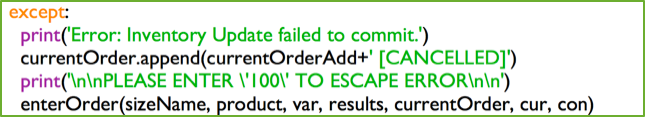
\includegraphics{task2_obj6_1.png} \par
If the user enters an invalid number, the \verb|sqlite3| library may get confused, and may enter an error loop. To break this loop, the user has to force the library to send another invalid request to the database.

\newpage
\subsection{Task 3}
\paragraph{Objective 1: Scan a database and find stock to order} ~\par ~\par
\noindent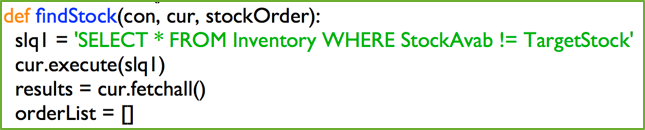
\includegraphics{task3_obj1_1.png} \par 
The \verb|findStock()| function sends a SQL query to the database to find any record where the stock level does not equal the target stock level. It then sets the variable \verb?results? to these results.
\paragraph{Objective 2: Create a receipt of the order} ~\par ~\par
\noindent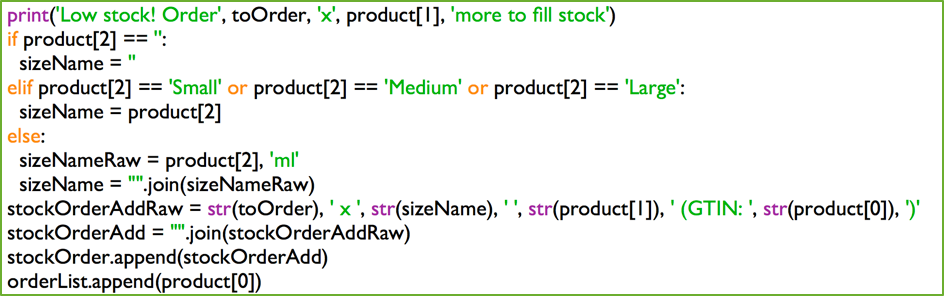
\includegraphics{task3_obj2_1.png} \par 
This section is similar to Task 2 Objective 4, and formats a verbose name of the product, and adds it to the receipt list.
\paragraph{Objective 3: Update the database with the updated stock level} ~\par ~\par
\noindent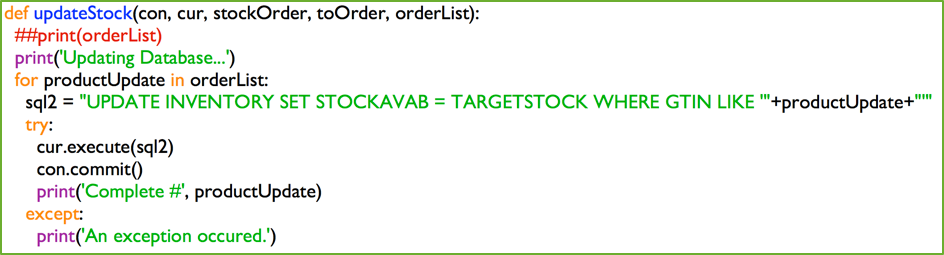
\includegraphics{task3_obj3_1.png} \par 
This function connects to the SQL database and updates the new stock levels. If it fails, it returns to the last function. 
\paragraph{Objective 4: Cope with any SQL errors} ~\par ~\par
\noindent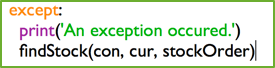
\includegraphics{task3_obj4_1.png} \par 
There should not be any SQL errors, as the user does not input any information that is used directly in the SQL query. This also protects against SQL injection.

%%%%%%%%%%%%%%%%%%%%%%%%%%%%%%%%%%%%%%%%%%%%%%%%%%%%%%%%%%%%%%%%%%%%%%%%%%%%
\newpage

\section{Testing}
\subsection{Task 1}
\paragraph{Test 1: Input strings of incorrect length. If rejected, it passes} ~\par
\noindent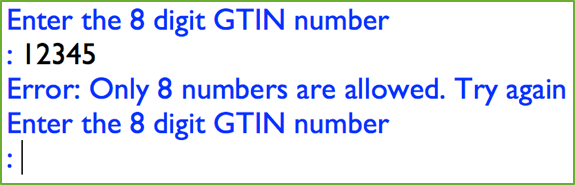
\includegraphics{testing_1.png} \par 
\noindent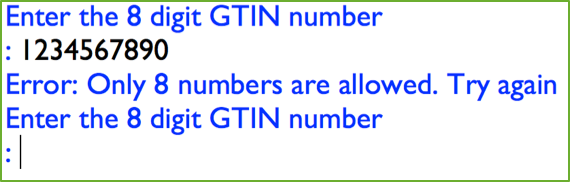
\includegraphics{testing_2.png} \par 
These show that the length verification is working.
\paragraph{Test 2: Input strings of letters. If rejected, it passes} ~\par 
\noindent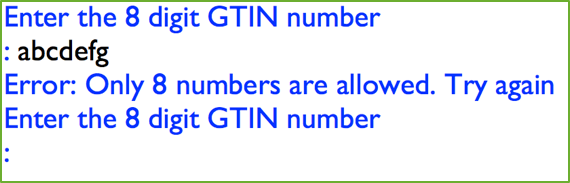
\includegraphics{testing_3.png} \par 
This shows that the numerical verification is working
\paragraph{Test 3: Get program to run a valid input. Print out totals at each stage, and check them manually. If they are the same, it passes}~\par ~\par 
\noindent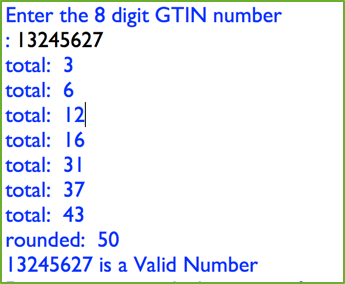
\includegraphics{testing_4.png} \par 
\noindent 1*3 = 3 \\
3+3*1=6 \\
6+2*3=12 \\ 
12+4*1=16 \\
16+5*3=31 \\
31+6*1=37 \\
37+2*3=43 \\
Highest 10 of 43 = 50 \\
50-43 = 7 \\ 
Checkdig = 7 \\
\paragraph{Test 4: Run the program with a GTIN number taken from a product. If it correctly calculated and verified, it passes}~\par ~\par 
\noindent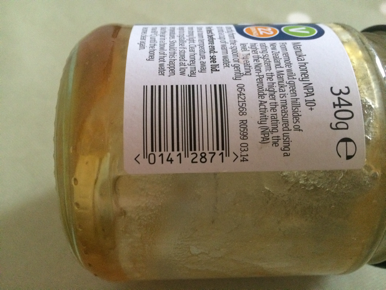
\includegraphics{testing_5.png} 
\noindent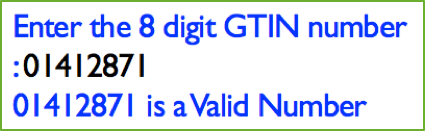
\includegraphics{testing_6.png} \par 
This shows that my program works in a real world situation, and can easily verify or calculate real GTIN codes.

\subsection{Task 2}	
\paragraph{Test 1: Input strings of incorrect length. If rejected, it passes} ~\par ~\par
\noindent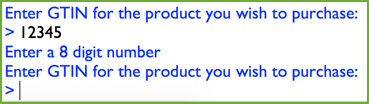
\includegraphics{testing_7.png} 
\noindent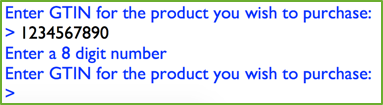
\includegraphics{testing_8.png} \par 
From these, you can see that my length verification is working.
\paragraph{Test 2: Input strings of letters. If rejected, it passes} ~\par ~\par
\noindent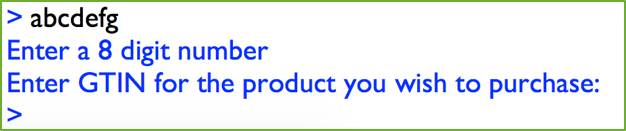
\includegraphics{testing_9.png} \par
From this, you can see that my numerical verification is working.
\paragraph{Test 3: Input a valid string to search. If product found, it passes} ~\par ~\par
\noindent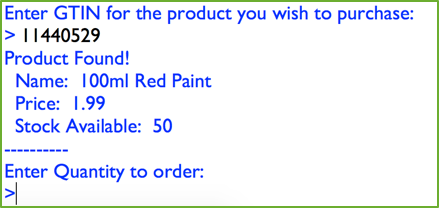
\includegraphics{testing_10.png} \par
The program successfully located a valid product
\newpage
\paragraph{Test 4: Manually check that the program has displayed the correct stock level and information. If it has, it passes.} ~\par ~\par
\noindent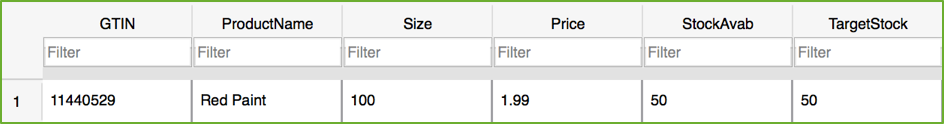
\includegraphics{testing_11.png} \par
The program has displayed the correct information for product \verb|#11440529|
\paragraph{Test 5: Order a quantity of the product. If the program updates the stock levels, it passes.} ~\par ~\par
\noindent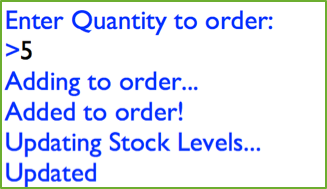
\includegraphics{testing_12.png}
\noindent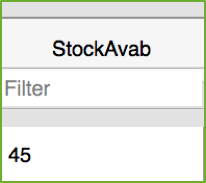
\includegraphics{testing_13.png} \par
The program successfully ordered 5 of \verb|#11440529| and updated the database
\paragraph{Test 6: Complete a full order. If the program displays a receipt with the correct values, it passes} ~\par ~\par
\noindent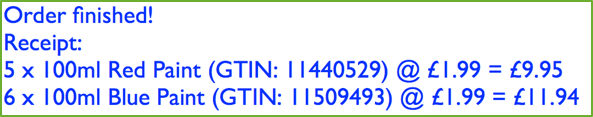
\includegraphics{testing_14.png}
The program successfully ordered the products, printed a receipt, and calculated the correct cost.
\paragraph{Test 7: Provide the program with invalid values (such as ordering negative values). If the program rejects these, it passes.} ~\par ~\par
\noindent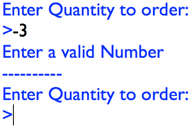
\includegraphics{testing_15.png}
\noindent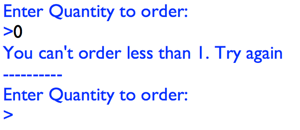
\includegraphics{testing_16.png}
\noindent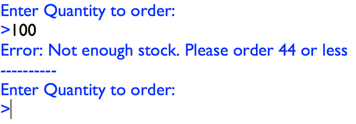
\includegraphics{testing_17.png} \par
This shows that the program rejects negative and 0 quantities, as well as quantities above the stock level. 
\newpage
\subsection{Task 3}
\paragraph{Test 1: Edit database for reduced stock. If reduced stock is identified, it passes} ~\par ~\par
%testing_18.png is missing
\noindent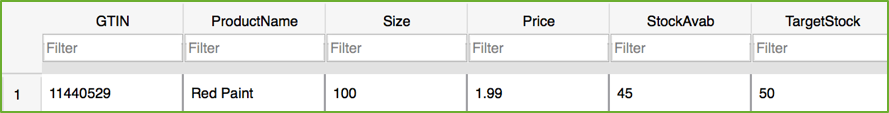
\includegraphics{testing_19.png} \par
\noindent
\includegraphics{testing_20.png} \par
This shows that the program can correctly identify a reduced stock
\paragraph{Test 2: Edit database for reduced stock. If a human-readable receipt is produced, it passes} ~\par ~\par
\noindent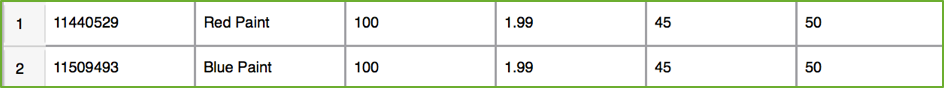
\includegraphics{testing_21.png} \par
\noindent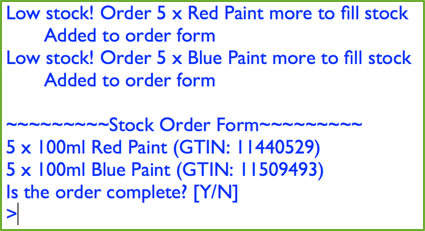
\includegraphics{testing_22.png} \par
This shows that the program can correctly identify two reduced stock levels, and append them to a verbose receipt
\paragraph{Test 3: Complete order for reduced stock. If the database updated, it passes.} ~\par ~\par
\noindent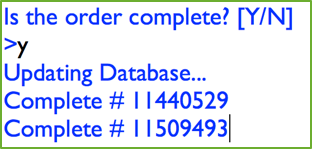
\includegraphics{testing_23.png}
\noindent\includegraphics{testing_24.png} \par
This shows that the program can update the database with the new stock level
\paragraph{Test 4: If the program handles SQL errors, it passes} ~\par ~\par
\noindent\includegraphics{testing_24.png} \par
The program does not allow the user to order any stock if all stock levels are up to date
\newpage

%%%%%%%%%%%%%%%%%%%%%%%%%%%%%%%%%%%%%%%%%%%%%%%%%%%%%%%%%%%%%%%%%%%%%%%%%%%%

\section{Final Program Code}
\subsection{Task 1}
\noindent\includegraphics[width=1\textwidth, left]{task1FINALCODE.png} \par 
\newpage
\subsection{Task 2}
\noindent\includegraphics[width=1\textwidth, left]{task2FINALCODE1.png} \par
\noindent\includegraphics[width=1.039\textwidth, left]{task2FINALCODE2.png} \par
\noindent\includegraphics[width=0.85\textwidth, left]{task2FINALCODE3.png}
\newpage
\subsection{Task 3}
\noindent\includegraphics[width=1\textwidth, left]{task3FINALCODE1.png} \par
\noindent\includegraphics[width=0.955\textwidth, left]{task3FINALCODE2.png} \par




\end{document}